\documentclass[12pt]{report}
\usepackage[utf8]{inputenc}
\usepackage[russian]{babel}
%\usepackage[14pt]{extsizes}
\usepackage{listings}
\usepackage{graphicx}
\usepackage{amsmath,amsfonts,amssymb,amsthm,mathtools} 
\usepackage{pgfplots}
\usepackage{filecontents}
\usepackage{indentfirst}
\usepackage{eucal}
\usepackage{amsmath}
\usepackage{enumitem}
\frenchspacing

\usepackage{indentfirst} % Красная строка


%\usetikzlibrary{datavisualization}
%\usetikzlibrary{datavisualization.formats.functions}

\usepackage{amsmath}


% Для листинга кода:
\lstset{ %
language=haskell,                 % выбор языка для подсветки (здесь это С)
basicstyle=\small\sffamily, % размер и начертание шрифта для подсветки кода
numbers=left,               % где поставить нумерацию строк (слева\справа)
numberstyle=\tiny,           % размер шрифта для номеров строк
stepnumber=1,                   % размер шага между двумя номерами строк
numbersep=5pt,                % как далеко отстоят номера строк от подсвечиваемого кода
showspaces=false,            % показывать или нет пробелы специальными отступами
showstringspaces=false,      % показывать или нет пробелы в строках
showtabs=false,             % показывать или нет табуляцию в строках
frame=single,              % рисовать рамку вокруг кода
tabsize=2,                 % размер табуляции по умолчанию равен 2 пробелам
captionpos=t,              % позиция заголовка вверху [t] или внизу [b] 
breaklines=true,           % автоматически переносить строки (да\нет)
breakatwhitespace=false, % переносить строки только если есть пробел
escapeinside={\#*}{*)}   % если нужно добавить комментарии в коде
}

\usepackage[left=2cm,right=2cm, top=2cm,bottom=2cm,bindingoffset=0cm]{geometry}
% Для измененных титулов глав:
\usepackage{titlesec, blindtext, color} % подключаем нужные пакеты
\definecolor{gray75}{gray}{0.75} % определяем цвет
\newcommand{\hsp}{\hspace{20pt}} % длина линии в 20pt
% titleformat определяет стиль
\titleformat{\chapter}[hang]{\Huge\bfseries}{\thechapter\hsp\textcolor{gray75}{|}\hsp}{0pt}{\Huge\bfseries}


% plot
\usepackage{pgfplots}
\usepackage{filecontents}
\usetikzlibrary{datavisualization}
\usetikzlibrary{datavisualization.formats.functions}

\begin{document}
%\def\chaptername{} % убирает "Глава"
\thispagestyle{empty}
\begin{titlepage}
	\noindent \begin{minipage}{0.15\textwidth}
	
\includegraphics[width=\linewidth]{b_logo}
	\end{minipage}
	\noindent\begin{minipage}{0.9\textwidth}\centering
		\textbf{Министерство науки и высшего образования Российской Федерации}\\
		\textbf{Федеральное государственное бюджетное образовательное учреждение высшего образования}\\
		\textbf{~~~«Московский государственный технический университет имени Н.Э.~Баумана}\\
		\textbf{(национальный исследовательский университет)»}\\
		\textbf{(МГТУ им. Н.Э.~Баумана)}
	\end{minipage}
	
	\noindent\rule{18cm}{3pt}
	\newline\newline
	\noindent ФАКУЛЬТЕТ $\underline{\text{«Информатика и системы управления»}}$ \newline\newline
	\noindent КАФЕДРА $\underline{\text{«Программное обеспечение ЭВМ и информационные технологии»}}$\newline\newline\newline\newline\newline
	
	
	\begin{center}
		\noindent\begin{minipage}{1.3\textwidth}\centering
			\Large\textbf{  Отчёт по лабораторной работе №5}\newline
			\textbf{по дисциплине "Анализ алгоритмов"}\newline\newline
		\end{minipage}
	\end{center}
	
	\noindent\textbf{Тема} $\underline{\text{Конвейерные вычисления}}$\newline\newline
	\noindent\textbf{Студент} $\underline{\text{Романов А.В.}}$\newline\newline
	\noindent\textbf{Группа} $\underline{\text{ИУ7-53Б}}$\newline\newline
	\noindent\textbf{Преподаватели} $\underline{\text{Волкова Л.Л., Строганов Ю.В.}}$\newline\newline\newline
	
	\begin{center}
		\vfill
		Москва~---~\the\year
		~г.
	\end{center}
\end{titlepage}


\tableofcontents

\newpage
\chapter*{Введение}
\addcontentsline{toc}{chapter}{Введение}

При обработке данных могут возникать ситуации, когда один набор данных необходимо обработать последовательно несколькими алгоритмами. В таком случае удобно использовать конвейерную обработку данных, что позволяет на каждой следующей <<линии>> конвейера использовать данные, полученные с предыдущего этапа. 

Помимо линейной конвейерной обработки данных, существуют асинхронная конвейерная обработка данных. При таком подходе все линии работают с меньшим времени простоя, так как могут обрабатывать задачи независимо от других линий.

\section*{Цель лабораторной работы}

Целью данной лабораторной работы является изучение и реализация асинхронной конвейерной обработки данных.

\section*{Задачи лабораторной работы}

В рамках выполнения работы необходимо решить следующие задачи:

\begin{itemize}
	\item изучить асинхронную конвейерную обработку данных;
	\item реализовать систему конвейерных вычислений с количеством линий не меньше трёх;
	\item сделать выводы на основе проделанной работы.
\end{itemize}

\chapter{Аналитическая часть}

В данном разделе представленные теоретические сведения о рассматриваемых алгоритмах.

\section{Конвейерная обработка данных}

Конвейер -- способ организации вычислений, используемый в современных процессорах и контроллерах с целью повышения их производительности (увеличения числа инструкций, выполняемых в единицу времени -- эксплуатация параллелизма на уровне инструкцией), технология, используемая при разработке компьютеров и других цифровых электронных устройств.

Идея заключается в параллельном выполнении нескольких инструкций процессора. Сложные инструкции процессора представляются в виде последовательности более простых стадий. Вместо выполнения инструкций последовательно, следующая инструкция может выполняться через несколько стадий выполнения первой инструкции. Это позволяет управляющим цепям процессора получать инструкции со скоростью самой медленной стадии обработки, однако при этом намного быстрее, чем при выполнении эксклюзивной полной обработки каждой инструкции от начала до конца.

Многие современные процессоры управляются тактовым генератором. Процессор внутри состоит из логических элементов и ячеек памяти -- триггеров. Когда приходит сигнал от тактового генератора, триггеры приобретают своё новое значение, и <<логике>> требуется некоторое время для декодирования новых значений. Затем приходит следующий сигнал от тактового генератора, триггеры принимают новые значения, и так далее. Разбивая последовательности логических элементов на более короткие и помещая триггеры между этими короткими последовательностями, уменьшают время необходимое логике для обработки сигналов. В этом случае длительность одного такта процессора может быть соответственно уменьшена.

\section{Описание задачи}

В качестве алгоритма, реализованного для распределения на конвейере, был выбран процес сборки автомобиля, состоящий из трех этапов:

\begin{itemize}
	\item сборка движка (возведение числа в степень);
	\item сборка корпуса (проверка числа на простоту);
	\item сборка колёс (вычисление числа Фибоначчи).
\end{itemize}

\section*{Вывод}
	В данном разделе были рассмотренны особенности построения конвейерных вычислений.

\chapter{Конструкторская часть}

В данном разделе представлены схемы рассматриваемых алгоритмов.

\section{Разработка алгоритмов}

На рисунке 2.1 приведена схема организации конвейерных вычислений.

\begin{figure}[h]
	\centering
	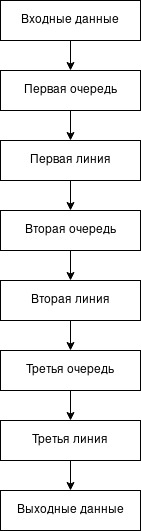
\includegraphics[scale=0.6]{scheme_lab05.jpg}
	\caption{Схема организации конвейерных вычислений.}
	\label{fig:mpr}
\end{figure}


\section*{Вывод}
На основе теоретических данных, полученных аз аналитического раздела, были построенна схема алгоритма конвейерных вычислений.

\chapter{Технологическая часть}

В данном разделе приведены средства реализации и листинги кода.

\section{Требование к ПО}

К программе предъявляется ряд требований:

\begin{itemize}
	\item на вход подается количество задач (количество машин, которые нужно собрать)
	\item на выходе -- время, затраченное на обработку заявок;
	\item в процессе обрабатывания задач необходимо фиксировать время прихода и ухода заявки с линии.
\end{itemize}

\section{Средства реализации}

Для реализации ПО я выбрал язык программирования С++ \cite{C++}. Данный выбор обусловлен высокой скоростью работы языка, а так же наличия инструментов для создания и эффективной работы с потоками.

\section{Реализация алгоритмов}

В листингах 3.1 и 3.2 приведены реализации конвейерных вычислений (класс Cloveyor), реализация сборки машины (класс Car) и реализация класса отвечающего за логгирование (класс Logger).

\begin{lstlisting}[label=some-code,caption=Реализация класса конвейера, language=C++]
#include <thread>
#include <queue>

#include "car.h"

#define THRD_CNT 3

class Conveyor
{
public:
	Conveyor() = default;
	~Conveyor() = default;
	
	void run(size_t cars_cnt);
	
	void create_engine();
	void create_carcass();
	void create_wheels();
	
private:
	std::thread threads[THRD_CNT];
	std::vector<std::shared_ptr<Car>> cars;
	
	std::queue<std::shared_ptr<Car>> q1;
	std::queue<std::shared_ptr<Car>> q2;
	std::queue<std::shared_ptr<Car>> q3;
};

void Conveyor::run(size_t cars_cnt)
{
	for (size_t i = 0; i < cars_cnt; i++)
	{
		std::shared_ptr<Car> new_car(new Car);
		cars.push_back(new_car);
		q1.push(new_car);
	}
	
	this->threads[0] = std::thread(&Conveyor::create_carcass, this);
	this->threads[1] = std::thread(&Conveyor::create_engine, this);
	this->threads[2] = std::thread(&Conveyor::create_wheels, this);
	
	for (int i = 0; i < THRD_CNT; i++)
	{
		this->threads[i].join();
	}
}

void Conveyor::create_carcass()
{
	size_t task_num = 0;
	
	while (!this->q1.empty())
	{
		std::shared_ptr<Car> car = q1.front();
		car->create_carcass(++task_num);
		
		q2.push(car);
		q1.pop();
	}
}

void Conveyor::create_engine()
{
	size_t task_num = 0;
	
	do
	{
		if (!this->q2.empty())
		{
			std::shared_ptr<Car> car = q2.front();
			car->create_engine(++task_num);
	
			q3.push(car);
			q2.pop();
		}
	} while(!q1.empty() || !q2.empty());
}

void Conveyor::create_wheels()
{
	size_t task_num = 0;
	
	do
	{
		if (!this->q3.empty())
		{
			std::shared_ptr<Car> car = q3.front();
			car->create_wheels(++task_num);
			q3.pop();
		}
	} while (!q1.empty() || !q2.empty() || !q3.empty());
}
\end{lstlisting}

\begin{lstlisting}[label=some-code,caption=Реализация класса сборки машины, language=C++]
#include <memory>
#include <cmath>

#include "logger.h"

class Carcass
{
public:
	Carcass(size_t num);
	~Carcass() = default;
	
	bool is_freight;
};

class Engine
{
public:
	Engine(int a, int x);
	~Engine() = default;
	
	size_t engine_power;
};

class Wheels
{
public:
	Wheels(int n);
	~Wheels() = default;
	
	size_t wheels_cnt;
};

class Car
{
public:
	Car() = default;
	~Car() = default;
	
	void create_engine(size_t);
	void create_carcass(size_t);
	void create_wheels(size_t);
	
private:
	std::unique_ptr<Carcass> carcass;
	std::unique_ptr<Engine> engine;
	std::unique_ptr<Wheels> wheels;
};

Carcass::Carcass(size_t num)
{
	this->is_freight = false;
	
	for (size_t i = 2; i <= sqrt(num); i++)
	{
		if (0 == num % i)
		{
			return;
		}
	}
	
	this->is_freight = true;
}

Engine::Engine(int a, int x)
{    
	this->engine_power = a;
	
	for (int i = 0; i < x; i++)
	{
		this->engine_power *= a;
	}
}

Wheels::Wheels(int n)
{
	size_t f1 = 1, f2 = 1;
	this->wheels_cnt = f1;
	
	for (int i = 2; i < n; i++)
	{
		this->wheels_cnt = f1 + f2;
		f1 = f2;
		f2 = this->wheels_cnt;
	}
}

void Car::create_engine(size_t task_num)
{
	Logger::log_current_event(task_num, "Part 2 | Start");
	
	if (this->carcass->is_freight) 
	{
		this->engine = std::unique_ptr<Engine>(new Engine(10, 150000));
	} 
	else
	{
		this->engine = std::unique_ptr<Engine>(new Engine(5,  150000));
	}

	Logger::log_current_event(task_num, "Part 2 | End  ");
}

void Car::create_carcass(size_t task_num)
{
	Logger::log_current_event(task_num, "Part 1 | Start");
	this->carcass = std::unique_ptr<Carcass>(new Carcass(27644437));
	Logger::log_current_event(task_num, "Part 1 | End  ");
}

void Car::create\_wheels(size\_t task\_num)
{
	Logger::log_current_event(task_num, "Part 3 | Start");
	this->wheels = std::unique_ptr<Wheels>(new Wheels(this->engine->engine\_power));
	Logger::log_current_event(task_num, "Part 3 | End  ");
}
\end{lstlisting}

\begin{lstlisting}[label=some-code,caption=Реализация класса логирования, language=C++]
#include <iostream>
#include <chrono>

using namespace std::chrono;

class Logger 
{
public:
	Logger() = default;
	~Logger() = default;
	
	static void log_current_event(size_t task_num, const char *const event);
}

void Logger::log_current_event(size_t task_num, const char *const event) 
{
	system_clock::time_point now = system_clock::now();
	system_clock::duration tp = now.time_since_epoch();
	
	tp -= duration_cast<seconds>(tp);
	
	time_t tt = system_clock::to_time_t(now);
	tm t = *gmtime(&tt);
	
	std::printf(
		"Task #%lu | %s | %02u:%02u:%02u.%3u\n", 
		task_num,
		event, 
		t.tm_hour, 
		t.tm_min, 
		t.tm_sec, 
		static_cast<unsigned>(tp / milliseconds(1))
	);
}
\end{lstlisting}

%\section{Тестовые данные}

\section*{Вывод}

В данном разделе была разработана и рассмотрена реализация конвейерных вычислений.

\chapter{Исследовательская часть}

В данном разделе приведен анализ характеристик разработанного ПО  и примеры работы ПО.

\section{Пример работы программы}

\begin{figure}[h]
	\centering
	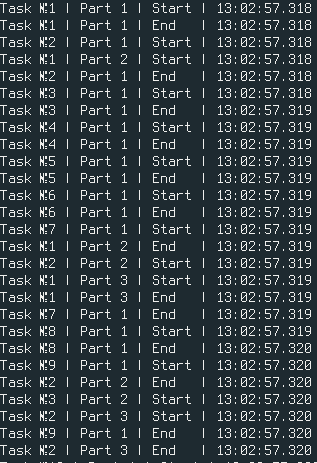
\includegraphics[scale=0.8]{prog_ex.png}
	\caption{Пример работы программы}
	\label{fig:mpr}
\end{figure}

\section{Технические характеристики}

Ниже приведены технические характеристики устройства, на котором было проведено тестирование ПО:

\begin{itemize}
	\item Операционная система: Debian \cite{debian} Linux \cite{linux} 11 <<bullseye>> 64-bit.
	\item Оперативная память: 12 GB.
	\item Процессор: Intel(R) Core(TM) i5-3550 CPU @ 3.30GHz
\cite{i5}.

\end{itemize}

\section{Время выполнения алгоритмов}

Время выполнения алгоритма замерялось с помощью применения технологии профайлинга \cite{profiling}. Данный инструмент даёт детальное описание количество вызовов и количества времени CPU, затраченного на выполнение каждой функции.

\begin{table} [h!]
	\caption{Таблица времени выполнения асинхронной обработки данных}
	\begin{center}
		\begin{tabular}{|c c c c c|} 
		 	\hline
			Количество задач & Линия №1 & Линия №2 & Линия №3 & Общее время работы  \\  
		 	\hline
		 	50 & 0.03 & 0.16 & 0.01 & 0.27 \\
		 	\hline
		 	100 & 0.06 & 0.34 & 0.02 & 0.47 \\
		 	\hline
		 	200 & 0.13 & 0.63 & 0.06 & 0.9 \\
		 	\hline
			400 & 0.3 & 1.32 & 0.15 & 1.86 \\
			\hline
			800 & 0.63  & 2.45 & 0.31 & 3.45 \\
			\hline
		\end{tabular}
	\end{center}
\end{table}

В таблице 4.1 приведено сравнение времени выполнения асинхронной обработки данных (сборка машины), в зависимости от количества входных задач (количества машин). Линия №1 - сборка каркасов автомобилей (проверка числа на простоту), линия №2 - сборка двигателей автомобилей (возведение числа в степень), линия №3 - сборка колёс автомобилей (вычисление числа Фибоначчи).

\section*{Вывод}

В данном разделе приведены время исполнения алгоритмов. Как видно из таблицы 4.1, вторая линия, то есть сборка двигателей (возведение числа в степень) занимает в среднем 70\% времени от выполнения всей программы. Линия №3 в среднем работает быстрее чем линия №1.

\chapter*{Заключение}
\addcontentsline{toc}{chapter}{Заключение}

В рамках данной лабораторной работы лабораторной работы была достигнута её цель: изучена асинхронная конвейерная обработка данных. Также выполнены следующие задачи:

\begin{itemize}
	\item изучена асинхронная конвейерная обработка данных
	\item реализована система конвейерных вычислений с количеством линий не меньше трёх;
	\item сделаны выводы на основе проделанной работы;
\end{itemize}

 Асинхронные конвейерные вычисления позволяют организовать непрерывную обработку данных, что позволяет выиграть время в задачах, где требуется обработка больших объемов данных за малый промежуток времени.

\addcontentsline{toc}{chapter}{Литература}

\bibliographystyle{utf8gost705u}  % стилевой файл для оформления по ГОСТу

\bibliography{51-biblio}          % имя библиографической базы (bib-файла)


\end{document}
